\documentclass[conference]{IEEEtran}
\IEEEoverridecommandlockouts
% Based on the IEEE conference template (Overleaf: "IEEE Conference Template").
\usepackage{cite}
\usepackage{amsmath,amssymb,amsfonts}
\usepackage{algorithm}
\usepackage{algorithmic}
\usepackage{graphicx}
\usepackage{textcomp}
\usepackage{xcolor}
\usepackage{booktabs}
\usepackage{capt-of}
\usepackage{url}
\usepackage{tikz}
\usetikzlibrary{arrows.meta,positioning,fit,backgrounds}
\usepackage{pgfplots}
\pgfplotsset{compat=1.18}
\def\BibTeX{{\rm B\kern-.05em{\sc i\kern-.025em b}\kern-.08em
    T\kern-.1667em\lower.7ex\hbox{\sc e}\kern-.125emX}}

% Shared bar-chart style for the benchmark figures
\pgfplotsset{benchbar/.style={
    ybar, width=\columnwidth, height=3.9cm, bar width=10pt,
    symbolic x coords={XDP,TC,TC+FIB,Kernel,nft+IPVS,OVS,OVS-ct}, xtick=data,
    ymin=0, enlarge x limits=0.13, axis lines*=left,
    ymajorgrids, grid style={gray!25},
    nodes near coords, every node near coord/.append style={font=\scriptsize},
    tick label style={font=\scriptsize}, label style={font=\footnotesize}}}

\ifdefined\pdfinfo
\pdfinfo{
  /Title (In-Kernel Programmable Data Planes for SDN: An eBPF/XDP Gateway with Stateful Firewalling and L4 Load Balancing Compared with Open vSwitch)
  /Subject (SDN data plane; eBPF/XDP gateway evaluation with supplementary figures)
  /Keywords (SDN, eBPF, XDP, load balancing, stateful firewall, Open vSwitch, nftables, IPVS)
}
\fi

\begin{document}

\title{In-Kernel Programmable Data Planes for SDN:\\
An eBPF/XDP Gateway with Stateful Firewalling and\\
L4 Load Balancing Compared with Open vSwitch}

% \author{\IEEEauthorblockN{Team 0}
% \IEEEauthorblockA{\textit{Department of Computer Science and Engineering} \\
% \textit{Indian Institute of Information Technology Dharwad}\\
% Dharwad, India \\
% patilyogeshgouda@gmail.com}}

\maketitle

\begin{abstract}
Software-Defined Networking (SDN) classically separates a controller from
switches that execute OpenFlow match--action tables. Cloud-native platforms
increasingly move this data plane into the operating-system kernel using the
extended Berkeley Packet Filter (eBPF) and the eXpress Data Path (XDP). This
paper designs, formally specifies, implements and evaluates such a data plane
for a gateway that combines a stateful firewall, a Layer-4 load balancer with
destination and source network address translation (DNAT/SNAT) and graceful
backend draining, and per-flow telemetry, in a single verified eBPF program
attachable at the XDP or the Traffic Control (TC) hook. A Python control plane
programs it at runtime through pinned BPF maps and a REST interface and
expires connection state like OpenFlow timeouts. The firewall judges
load-balanced traffic by the flow the client sees, which keeps VIP policies
consistent in both directions and keeps backends unreachable except through
the VIP. The implementation passes 115 of 116 automated unit and kernel tests
(one skipped by a kernel test-harness limitation), including packet tests
that check every rewritten checksum. We compare it with plain kernel routing,
the kernel's native stateful stack (nftables and IPVS), and Open vSwitch
(OVS) with stateless OpenFlow~1.3 rules and with connection tracking, over 10
interleaved, CPU-pinned rounds on emulated veth links, on a routed path and
through the load balancer. All stateful configurations provide the required
functions and spread load evenly, and all cost 13.6--26.9\% of throughput
relative to plain routing. With sparse rule sets, the eBPF data plane at the
TC hook is statistically indistinguishable from OVS with connection tracking
and, with in-program forwarding, 16--18\% faster than nftables with IPVS
through the virtual IP; at the XDP hook on veth it is 13\% below the latter
in packet rate. In-kernel microbenchmarks show a per-packet cost of 74--100~ns
with empty rule tables and 250--295~ns with all ten rule patterns populated,
independent of the number of rules (10--10\,000) and tracked connections
(0--60\,000), rising to about 0.68~$\mu$s when 60\,000 flows miss the cache.
Chaining the same stages with tail calls costs 33--47\% more on the pass
and NAT paths.
\end{abstract}

\begin{IEEEkeywords}
software-defined networking, eBPF, XDP, programmable data plane, load
balancing, stateful firewall, Open vSwitch, Mininet
\end{IEEEkeywords}

%=====================================================================
\section{Introduction}
%=====================================================================
SDN decouples the control plane, which decides how traffic should be handled,
from the data plane, which applies those decisions packet by packet
\cite{kreutz2015sdn,feamster2014road}. OpenFlow \cite{mckeown2008openflow}
standardized this split: a controller installs prioritized match--action
entries into the flow tables of switches such as Open vSwitch (OVS)
\cite{pfaff2015ovs}. The standard model is expressive for stateless
forwarding; stateful functions such as connection tracking and NAT are
provided through extensions, e.g., the \texttt{ct} and \texttt{nat} actions
of OVS backed by the kernel's connection tracker.

Cloud-native infrastructures have taken a different path. eBPF allows verified
programs to be loaded into a running Linux kernel and attached to networking
hooks, and XDP runs such programs in the network driver before the kernel
allocates its packet structure \cite{hoiland2018xdp,vieira2020ebpf}.
Production systems such as Cilium \cite{cilium} and Katran \cite{katran}, and
research frameworks such as Polycube \cite{miano2021polycube}, implement their
data planes this way. The controller--switch boundary of SDN thus becomes a
boundary between a user-space agent and kernel tables (BPF maps).

This paper does not claim the first eBPF implementation of a firewall or load
balancer---prior systems provide these functions (Section~\ref{sec:related}). Instead it
contributes a compact, \emph{formally specified} gateway pipeline and a
like-for-like comparison against the stateful alternatives available on the
same kernel. Our contributions are:
\begin{enumerate}
\item A single eBPF pipeline, attachable at the XDP or TC hook without
tail-call chaining (which our ablation shows saves 25--32\% of the
per-packet cost on the pass and NAT paths), that parses Ethernet/VLAN/ARP/IPv4/TCP/UDP/ICMP, enforces
a stateful firewall over MAC and IPv4 rules, load-balances connections to a
virtual IP (VIP) with DNAT/SNAT and graceful backend draining, and maintains
per-flow telemetry (Section~\ref{sec:method}).
\item A formal model of rule matching, stateful admission over the
client-visible flow, backend selection, NAT state coupling, checksum
maintenance and connection expiry, which is exactly the logic the
implementation executes (Section~\ref{sec:model}).
\item A libbpf-based control plane with a CLI, a REST API and a connection
reaper analogous to OpenFlow idle and hard timeouts.
\item An evaluation against four baselines---plain kernel routing, the
kernel's native stateful subsystems (nftables with connection tracking and
IPVS), stateless OpenFlow~1.3 on OVS, and OVS with connection tracking---with
116 automated tests, repeated and interleaved benchmark runs on a routed
path and through the load balancer with confidence intervals, and in-kernel
microbenchmarks of per-packet cost versus rule count, connection-table
occupancy and cache state, including a tail-call ablation (Sections~\ref{sec:setup}--\ref{sec:results}).
\end{enumerate}

%=====================================================================
\section{Related Work}
\label{sec:related}
%=====================================================================
\textit{SDN, OpenFlow and OVS.} Kreutz \textit{et al.}\ survey the SDN
architecture and its data-plane abstractions \cite{kreutz2015sdn}; Feamster
\textit{et al.}\ trace its history \cite{feamster2014road}. OpenFlow
\cite{mckeown2008openflow} defines the match--action switch model that OVS
\cite{pfaff2015ovs} implements with a user-space slow path and a kernel flow
cache; P4 \cite{bosshart2014p4} generalizes the data plane to
protocol-independent pipelines. Tu \textit{et al.}\ revisit the OVS data path
after ten years, including its eBPF and \texttt{AF\_XDP} variants \cite{tu2021ovs}, and
Oko extends OVS with stateful BPF filters placed in the OpenFlow pipeline
\cite{chaignon2018oko}.

\textit{eBPF and XDP network functions.} H{\o}iland-J{\o}rgensen
\textit{et al.}\ present the design of XDP \cite{hoiland2018xdp}, and Vieira
\textit{et al.}\ survey eBPF and XDP \cite{vieira2020ebpf}. Miano
\textit{et al.}\ report lessons from building network services with eBPF
\cite{miano2018creating}, build bpf-iptables, which reproduces iptables
semantics with an eBPF classifier \cite{miano2019bpfiptables}, and generalize
these ideas in Polycube, a framework of chained eBPF network functions
(firewall, NAT, load balancer, router) with a REST control plane
\cite{miano2021polycube}. Scholz \textit{et al.}\ quantify eBPF packet
filtering in Linux \cite{scholz2018filtering}. Cilium \cite{cilium} and Katran
\cite{katran} are production eBPF data planes for Kubernetes networking and L4
load balancing.

\textit{Kernel subsystems and classification.} Linux provides stateful
filtering through Netfilter/nftables with the \texttt{nf\_conntrack}
connection tracker \cite{nftables} and L4 load balancing through IPVS
\cite{zhang2000lvs}. Its software \emph{flowtable} (\texttt{nf\_flow\_table})
offloads established connections, including their NAT bindings, to the
ingress hook, where their packets bypass routing and the forward chain
\cite{nfflowtable}---the kernel's own counterpart of in-program FIB
forwarding, which we therefore include as a baseline. Maglev \cite{eisenbud2016maglev} introduced consistent
hashing for software load balancers. Tuple Space Search
\cite{srinivasan1999tss} classifies packets by probing one exact-match hash
table per combination of wildcarded fields; our rule matcher is a fixed tuple
space with ten tuples (Section~\ref{sec:rules}).

\textit{Positioning.} Compared with Polycube and bpf-iptables, which favor
generality (arbitrary rule sets, chains of independent programs), our design
keeps all functions in one program and one set of maps, specifies their
interaction formally---in particular how firewall state, NAT state and
draining interact---and evaluates the result against the kernel's own
stateful subsystems and a stateful OVS configuration rather than only against
stateless forwarding. Merging network functions into one program is a
known optimization: KFuse merges chained eBPF programs after verification
\cite{kuo2022kfuse}, and Morpheus specializes data-plane code at run time to
the installed rules and traffic \cite{miano2022morpheus}; modular frameworks
also pass parsed metadata between stages instead of re-parsing. We choose a
single program primarily because one set of maps makes the coupling of
firewall and NAT state easy to specify and keep consistent, and we quantify
the performance effect with an ablation that chains the same stages by tail
calls, both with re-parsing and with shared parse metadata
(Section~\ref{sec:kernel-cost}). We do not benchmark Polycube, bpf-iptables,
KFuse or Morpheus themselves, which also differ in parsing, state layout and
rule semantics. Mininet \cite{lantz2010mininet} is used for emulation;
because emulated hosts share one kernel, the eBPF program under test is the
real kernel program.

%=====================================================================
\section{Problem Scenario and System Model}
\label{sec:model}
%=====================================================================
\subsection{Scenario}
A gateway connects a client subnet $\mathcal{C}=\{c_1,\dots,c_4\}$
(10.0.1.0/24) and a backend subnet $\mathcal{S}=\{s_1,\dots,s_4\}$
(10.0.2.0/24). A service is published at the VIP $v=10.100.0.1$, port 80, and
must be served by the backends. The gateway must (i) forward all inter-host
traffic, (ii) enforce operator-defined allow/drop rules, (iii) distribute new
connections to the VIP across healthy backends while keeping each connection
on one backend, (iv) let operators drain a backend without breaking its
established connections, and (v) export packet and byte counters. Rules and
backend pools change at runtime without reloading the data plane.

\subsection{System Model}
Fig.~\ref{fig:arch} shows the architecture. Every host has a dedicated veth
link to the gateway (\textit{routed access}: /32 host routes and proxy ARP),
so every packet between any two hosts traverses the gateway data plane. The
data plane is a set of kernel functions sharing eleven BPF maps; the control
plane reads and writes the same maps through the \texttt{bpf()} system call.
Table~\ref{tab:maps} maps the formal symbols used below to the maps.

\begin{figure}[t]
\centering
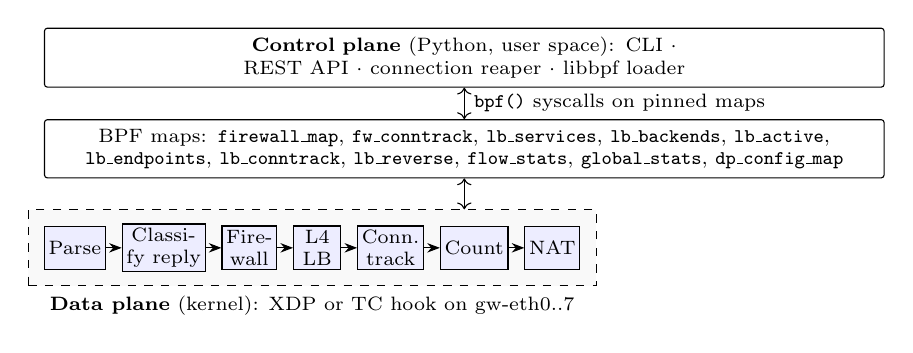
\begin{tikzpicture}[font=\scriptsize, node distance=2mm,
  box/.style={draw, rounded corners=1pt, align=center, minimum height=5mm, fill=white},
  stage/.style={draw, fill=blue!7, minimum height=5.5mm, minimum width=6mm, inner sep=1.5pt, align=center},
  arr/.style={-{Stealth[length=1.6mm]}}]
\node[box, text width=0.86\columnwidth] (cp) {\textbf{Control plane} (Python, user space):
  CLI $\cdot$ REST API $\cdot$ connection reaper $\cdot$ libbpf loader};
\node[box, below=4mm of cp, text width=0.86\columnwidth] (maps)
  {BPF maps: \texttt{firewall\_map}, \texttt{fw\_conntrack}, \texttt{lb\_services},
   \texttt{lb\_backends}, \texttt{lb\_active},\\ \texttt{lb\_endpoints},
   \texttt{lb\_conntrack}, \texttt{lb\_reverse}, \texttt{flow\_stats},
   \texttt{global\_stats}, \texttt{dp\_config\_map}};
\node[stage, below=6mm of maps.south west, anchor=north west, xshift=0mm] (p) {Parse};
\node[stage, right=of p] (r) {Classi-\\fy reply};
\node[stage, right=of r] (f) {Fire-\\wall};
\node[stage, right=of f] (l) {L4\\LB};
\node[stage, right=of l] (c) {Conn.\\track};
\node[stage, right=of c] (t) {Count};
\node[stage, right=of t] (n) {NAT};
\draw[arr] (p) -- (r); \draw[arr] (r) -- (f); \draw[arr] (f) -- (l); \draw[arr] (l) -- (c);
\draw[arr] (c) -- (t); \draw[arr] (t) -- (n);
\begin{scope}[on background layer]
\node[draw, dashed, fill=gray!5, inner sep=2mm, fit=(p)(n),
  label={[font=\scriptsize]below:\textbf{Data plane} (kernel): XDP or TC hook on gw-eth0..7}] (dp) {};
\end{scope}
\draw[arr, <->] (cp) -- node[right] {\texttt{bpf()} syscalls on pinned maps} (maps);
\draw[arr, <->] (maps.south) -- (maps.south |- dp.north);
\end{tikzpicture}
\caption{Architecture: a user-space control plane programs a kernel data
plane through shared BPF maps. ``Classify reply'' determines the rule key
(Eq.~(\ref{eq:kappa})) without changing state; ``L4 LB'' updates
$\mathcal{L}$ and $\mathcal{T}_{rev}$ only for admitted packets; ``Conn.\
track'' is the update of $\mathcal{T}_{fw}$ and ``NAT'' the header rewrite
(Algorithm~\ref{alg:pipeline}).}
\label{fig:arch}
\end{figure}

\begin{table}[t]
\caption{Formal symbols and their BPF maps (capacity in entries; the
per-service arrays hold 16 services $\times$ 16 slots)}
\label{tab:maps}
\centering\scriptsize
\setlength{\tabcolsep}{2.5pt}
\begin{tabular}{@{}llrl@{}}
\toprule
Symbol & Map (type) & Cap. & Content \\
\midrule
$\mathcal{R}$ & \texttt{firewall\_map} (hash) & 16\,384 & (pattern id, fields) $\mapsto$ action, hits \\
$\mathcal{T}_{fw}$ & \texttt{fw\_conntrack} (LRU hash) & 65\,536 & tracked flows, times, TCP flags \\
$\sigma$ & \texttt{lb\_services} (hash) & 16 & $(v,p_v,\pi) \mapsto$ id, $n$, $n_{\mathrm{act}}$ \\
$B_\sigma$, $\alpha$ & \texttt{lb\_backends} (array) & 256 & address, port, active flag \\
$\lambda$ & \texttt{lb\_active} (array) & 256 & indices of active backends \\
$\mathcal{E}$ & \texttt{lb\_endpoints} (hash) & 256 & $(a_b,p_b,\pi) \mapsto (v,p_v,\sigma,j)$ \\
$\mathcal{L}$ & \texttt{lb\_conntrack} (LRU hash) & 65\,536 & client flow $\mapsto (b,j)$ \\
$\mathcal{T}_{rev}$ & \texttt{lb\_reverse} (LRU hash) & 65\,536 & reply key $\mapsto (v,p_v,\sigma,j)$ \\
-- & \texttt{flow\_stats} (per-CPU LRU) & 16\,384 & per-flow packets, bytes \\
-- & \texttt{global\_stats} (per-CPU array) & 15 & pipeline counters \\
$\delta$, $\gamma$ & \texttt{dp\_config\_map} (array) & 1 & default action, flags, pattern mask \\
\bottomrule
\end{tabular}
\end{table}

\subsection{Flows and Rules}
\label{sec:rules}
An IPv4 packet $x$ carries the flow key
\begin{equation}
f(x) = (s, d, p_s, p_d, \pi),
\end{equation}
with addresses $s,d$, ports $p_s,p_d$ and protocol $\pi$. Let $\rho(x)=1$ iff
$x$ is TCP or UDP and is not an IPv4 fragment (neither the More-Fragments flag
nor a fragment offset is set), i.e., iff its ports are known; otherwise
$p_s=p_d=0$. ICMP is therefore matched on $(s,d,\pi)$ only, and all fragments
of a datagram share one key (Section~\ref{sec:method} discusses fragments,
whose first fragment's ports are used only to drop it). The reverse key is $\bar f = (d, s, p_d, p_s,
\pi)$.

Rules follow ten \emph{patterns}. Pattern $i$ selects a subset of fields, and a
rule is stored under the key $(i, m_i(\cdot))$, where $i$ is the
\emph{pattern id}; because $i$ is part of the key, an unselected field is a
true wildcard and a packet whose port or protocol happens to be zero can never
match a wildcarded rule by accident. In lookup order:
\begin{equation}
\begin{aligned}
&m_1{:}\,(\mathrm{mac}_s,\mathrm{mac}_d),\;\; m_2{:}\,(\mathrm{mac}_s),\;\;
 m_3{:}\,(s,d,p_s,p_d,\pi)^{\rho},\\
&m_4{:}\,(s,d,p_d,\pi)^{\rho},\;\; m_5{:}\,(s,d,p_s,\pi)^{\rho},\;\;
 m_6{:}\,(s,d,\pi),\\
&m_7{:}\,(s,d),\;\; m_8{:}\,(d,p_d,\pi)^{\rho},\;\; m_9{:}\,(s),\;\;
 m_{10}{:}\,(d),
\end{aligned}
\label{eq:patterns}
\end{equation}
where $^{\rho}$ marks patterns that require $\rho(x)=1$. The L2 patterns
$m_1,m_2$ are functions of the Ethernet header and apply to every frame,
including IPv6 and other non-IP traffic; $m_3$--$m_{10}$ are functions of an
IPv4 key. With $I_2=\{1,2\}$ and $I_4(\rho)=\{3,\dots,10\}\setminus\{i: m_i
\text{ requires } \rho \land \rho=0\}$, the L2 and IPv4 decisions are
\begin{equation}
\begin{aligned}
A_2(x) &= a\big(i^*, m_{i^*}(x)\big),\\
i^* &= \min\{i \in I_2 : (i, m_i(x)) \in \mathcal{R}\},\\
A(k,\rho) &= a\big(j^*, m_{j^*}(k)\big),\\
j^* &= \min\{i \in I_4(\rho) : (i, m_i(k)) \in \mathcal{R}\},
\end{aligned}
\label{eq:match}
\end{equation}
with result $\textsc{none}$ if no pattern matches. $A$ depends on $\rho$
as well as on $k$, because an unfragmented packet with zero ports and a
fragment have the same key; below we write $A(k)$ for $A(k,\rho(x))$. The order is a total
priority order, like OpenFlow priorities: where two patterns are incomparable
in specificity ($m_4$/$m_5$, $m_9$/$m_{10}$) the earlier one wins, and an
operator who needs the opposite outcome adds a more specific rule. An L2
\textsc{allow} rule only exempts a frame from a broader L2 \textsc{drop}
(e.g., an $m_1$ \textsc{allow} under an $m_2$ \textsc{drop}); whether an IPv4
packet is admitted is decided by $A(k)$ alone, and L2 \textsc{drop} rules
do not flush connection state, which is keyed by IPv4 tuples. Pattern $m_8$ expresses a
service rule such as ``any client may reach $v$:80/TCP''. The data plane skips
patterns that hold no rule; this does not change $A$.

\subsection{Rule Key and Stateful Admission}
A load-balanced connection is judged in one orientation, client$\to$VIP, in
both directions. For a backend reply $x$ with $f(x)=(a_b,c,p_b,p_c,\pi)$,
i.e., $(d,p_d)=(c,p_c)$, the rule key restores the client's view:
\begin{equation}
\kappa(x) = \begin{cases}
(d, v, p_d, p_v, \pi) & \text{if $x$ replies to a tracked}\\
 & \text{LB connection to } (v,p_v),\\
f(x) & \text{otherwise}.
\end{cases}
\label{eq:kappa}
\end{equation}
Forward packets to the VIP already carry $(c, v, p_c, p_v, \pi)$, so a single
rule against the VIP---e.g., $m_8$ ``any client may reach $v$:80''---covers
both directions of the connection, even with the firewall's connection
tracking disabled ($\gamma=0$), since $\kappa$ uses only the load balancer's
tables; a rule between a client and a specific backend does not affect traffic through
the VIP; a broader rule such as $m_{10}$: $(d{=}c)\mapsto\textsc{drop}$ does
not hit replies, whose key has destination $v$; and no firewall state is ever
created for a backend's real address. For VIP traffic, the patterns are
therefore predicates on the \emph{connection} (e.g., $m_9$: $(s{=}c)$
matches both directions, $(s{=}v)$ neither), whereas all other traffic is
matched in the orientation in which it travels. Section~\ref{sec:coupling}
defines when a packet is a reply of a tracked load-balanced connection.

Let $\gamma\in\{0,1\}$ indicate whether connection tracking is enabled and
$\delta$ the default action. A flow is \emph{established} iff $E(k)=1$, where
$E(k) = \mathbb{1}\big[\gamma = 1 \land (k \in \mathcal{T}_{fw} \lor \bar k \in
\mathcal{T}_{fw})\big]$, so $E(k)=0$ when tracking is disabled. Non-IPv4
frames (ARP, IPv6, \dots) are admitted iff $A_2(x) \ne \textsc{drop}$,
independently of $\delta$, so IP policy cannot break address resolution. An
IPv4 packet with $k=\kappa(x)$ is admitted iff $A_2(x) \ne \textsc{drop}$ and
$\mathrm{adm}(x)=1$, where
\begin{equation}
\mathrm{adm}(x) =
\begin{cases}
0 & A(k) = \textsc{drop},\\
1 & A(k) = \textsc{allow},\\
1 & A(k) = \textsc{none} \land \delta=\textsc{allow},\\
E(k) & A(k) = \textsc{none} \land \delta = \textsc{drop}.
\end{cases}
\label{eq:adm}
\end{equation}
An explicit \textsc{drop} rule takes effect on the next packet in either
direction, even on established connections; when one is added, the control
plane additionally flushes the matching connection state. After an admitted
packet has also passed the load balancer, and if $\gamma=1$, the tracker
refreshes the entry of $k$ if $k\in\mathcal{T}_{fw}$, otherwise that of $\bar
k$ if present, and otherwise inserts $k$. A packet counts as a reply if it is
a load-balanced reply by Eq.~(\ref{eq:kappa})---its key $k$ then hits the
client's entry directly---or if only $\bar k$ is present (routed traffic);
a reply marks the entry as having seen a reply. Each connection thus occupies
one entry, with one pair of timestamps and the union of the TCP flags of both
directions; the timeout of Eq.~(\ref{eq:expiry}) needs only whether a FIN or
RST was seen, not by whom.

\subsection{Load-Balancing Model}
A service $\sigma=(v,p_v,\pi)$ owns an ordered backend pool
$B_\sigma=(b_0,\dots,b_{n-1})$ of size $n \le 16$, where each backend
$b_j=(a_j, p_j)$ has an address, a port and an active flag $\alpha_j\in\{0,1\}$
($1$: active, $0$: draining). A backend keeps its slot $j$ while it stays in
the pool; removing one leaves an empty slot rather than shifting the others,
because established connections refer to backends by slot.
Let $n_{\mathrm{act}} = \sum_{j=0}^{n-1}\alpha_j$ and let
$(\lambda_0,\dots,\lambda_{n_{\mathrm{act}}-1})$ be the indices of the active
backends in pool order. For a new connection $f$, the gateway computes a hash
$h(f)$ (Bob Jenkins' \textit{jhash} final mix over $s$, $d$ and the
port/protocol word) and selects
\begin{equation}
j^*(f) = \lambda_{\,h(f) \bmod n_{\mathrm{act}}}
\quad \text{if } n_{\mathrm{act}} > 0;
\label{eq:select}
\end{equation}
if $n_{\mathrm{act}} = 0$, the packet is dropped. The choice is stored as
$\mathcal{L}[f]=(b_{j^*}, j^*)$. Because the hash is taken modulo the number
of \emph{active} backends, draining a backend spreads its share evenly over
all remaining ones; a uniform $h$ gives every active backend an expected
$N/n_{\mathrm{act}}$ of $N$ new connections, which we test with Pearson's
statistic over the active backends,
\begin{equation}
\chi^2 = \sum_{j:\,\alpha_j=1} \frac{(N_j - N/n_{\mathrm{act}})^2}{N/n_{\mathrm{act}}},
\qquad \text{d.o.f.} = n_{\mathrm{act}}-1,
\label{eq:chi2}
\end{equation}
defined for $n_{\mathrm{act}} \ge 2$ (with one active backend the choice is
deterministic).

\textit{Stickiness and graceful draining.} For a later packet of $f$ with
$\mathcal{L}[f]=(b,j)$, the stored backend is reused as long as slot $j$ still
holds $b$ (same address and port), \emph{regardless of} $\alpha_j$: draining
($\alpha_j \gets 0$) removes $b_j$ from Eq.~(\ref{eq:select}) for new
connections only, while established connections continue until they close or
expire. Only if the backend was removed or replaced is $f$ re-selected; the
old backend's reverse entry $\mathcal{T}_{rev}[r_{b}(f)]$ is deleted first.
When a backend is removed or replaced, the control plane also flushes every
$\mathcal{L}$ and $\mathcal{T}_{rev}$ entry that names it, so no state
survives for a slot that now holds another backend.

\subsection{Address Translation, State Coupling and Recovery}
\label{sec:coupling}
For a client flow $f=(c,v,p_c,p_v,\pi)$ assigned to backend $b=(a_b,p_b)$, the
forward packet is rewritten by DNAT, $T_D(f)=(c,a_b,p_c,p_b,\pi)$, and the
reverse-NAT table records the key of the expected reply,
$\mathcal{T}_{rev}[r_b(f)] = (v,p_v,\sigma,j^*)$ with
$r_b(f)=(a_b,c,p_b,p_c,\pi)$; we write $r(f)$ when $b$ is the backend of
$\mathcal{L}[f]$. A reply matching this key is rewritten by SNAT to
$(v,c,p_v,p_c,\pi)$, so the client only ever observes the VIP.

\textit{Isolation.} A backend \emph{service endpoint} $(a_b,p_b,\pi)$ belongs
to exactly one service (the control plane rejects overlapping pools, per
address, port and protocol) and is reachable only through its VIP: a packet
addressed directly to a service endpoint is dropped, and so is the first
fragment of a datagram to or from one (Section~\ref{sec:method}). Hence no un-translated
connection can produce a key $r(f)$, and $\mathcal{T}_{rev}$ is injective. An
index $\mathcal{E}[(a_b,p_b,\pi)] = (v,p_v,\sigma,j)$ records each endpoint's
service.

\textit{Coupling and recovery.} $\mathcal{L}[f]$ and $\mathcal{T}_{rev}[r(f)]$
live in separate LRU maps and either can be lost to eviction or a reaper race
(Section~\ref{sec:reaper}). Each packet therefore refreshes both entries and
rebuilds a missing one from the other. Reply classification, which
determines $\kappa(x)$ before the firewall runs, is read-only; entries are
refreshed or re-created only after the packet has been admitted, so a packet
that the firewall drops never creates NAT state:
\begin{itemize}
\item a forward packet refreshes $\mathcal{L}[f]$ in place and refreshes or
re-creates $\mathcal{T}_{rev}[r(f)]$. If $\mathcal{L}[f]$ is missing and the
packet is not a TCP SYN, it probes $\mathcal{T}_{rev}[r_{b_i}(f)]$ for
$0 \le i < n$ (at most 16 lookups) and, on a hit recorded for slot $i$,
restores $\mathcal{L}[f]$ to $b_i$---even if it is draining. A SYN always
opens a new connection, so it is placed by Eq.~(\ref{eq:select}) and cannot
be captured by a leftover reverse entry of an earlier connection that used
the same client port; for UDP, which has no such signal, a leftover entry
can bind a new flow to its old backend until the entry expires;
\item a reply is classified as such if $\mathcal{T}_{rev}[f(x)] =
(v,p_v,\sigma,j)$ exists, or, if it is missing, if $\mathcal{E}$ yields
$(v,p_v,\sigma)$ and $\mathcal{L}[(c,v,p_c,p_v,\pi)] = (b,j)$ names this
backend; in both cases slot $j$ of $B_\sigma$ must still hold $(a_b,p_b)$.
After admission it refreshes or re-creates $\mathcal{T}_{rev}[f(x)]$ and
refreshes $\mathcal{L}[f]$, re-creating it from $(\sigma,j)$ if missing;
\item a packet from a service endpoint that fails these checks is dropped,
so a backend's real address can never reach a client.
\end{itemize}
Both directions record TCP FIN and RST flags (client flags in the forward
direction, server flags in replies), so either side's close shortens the
connection's timeout, and a server-to-client download keeps the connection
alive. A connection is lost only if both entries are lost before a packet
rebuilds one, as with any NAT that loses state.

\subsection{Incremental Checksum Maintenance}
Rewriting addresses and ports invalidates the IPv4 header checksum and the
TCP/UDP checksum, whose pseudo-header covers both addresses. Recomputing them
costs $O(L)$ for a packet of length $L$. We use the incremental update of
RFC~1624 \cite{rfc1624}: if 16-bit words $m_i$ change to $m_i'$,
\begin{equation}
HC' = {\sim}\Big({\sim}HC \oplus \textstyle\bigoplus_i {\sim}m_i
\oplus \bigoplus_i m_i'\Big),
\label{eq:csum}
\end{equation}
where $\oplus$ is 16-bit ones'-complement addition (end-around carry)
\cite{rfc1071} and ${\sim}$ is bitwise complement; the cost is $O(1)$. For
the IPv4 header the changed words are the two halves of one address; for the
L4 checksum they are the address (via the pseudo-header) and the port. The
implementation accumulates the sum in 32 bits with \texttt{bpf\_csum\_diff},
folds the carries into 16 bits and complements the result. The only special
case is UDP (RFC~768 \cite{rfc768}): a received checksum of zero (``not
computed'') is left unchanged, and a computed UDP checksum of
\texttt{0x0000} is transmitted as \texttt{0xFFFF}; IPv4 header and TCP
checksums are written as computed.

\subsection{Connection Expiry}
Each tracked entry $e$ stores its creation time $\tau_c(e)$, last-seen time
$\tau_\ell(e)$ (both from \texttt{bpf\_ktime\_get\_ns}) and the TCP flags seen
in either direction. With the idle limit $\Theta(e) = T_{\mathrm{fin}}$ if FIN
or RST has been seen and $T_{\mathrm{idle}}$ otherwise, the entry is removed at
reaper time $t$ iff
\begin{equation}
t - \tau_\ell(e) > \Theta(e)
\;\lor\; \big(T_{\mathrm{hard}} > 0 \,\land\, t - \tau_c(e) > T_{\mathrm{hard}}\big),
\label{eq:expiry}
\end{equation}
which mirrors OpenFlow's \texttt{idle\_timeout} and \texttt{hard\_timeout}.
Removing $\mathcal{L}[f]$ also removes $\mathcal{T}_{rev}[r(f)]$.

%=====================================================================
\section{Proposed Methodology}
\label{sec:method}
%=====================================================================
\subsection{Data-Plane Pipeline}
Algorithm~\ref{alg:pipeline} gives the per-packet processing. It is written
once and called by both entry points (\texttt{xdp\_dataplane} and
\texttt{tc\_dataplane}); only the final rewrite differs between hooks. Every
header access is preceded by an explicit bounds check against the end of the
packet, which lets the in-kernel verifier prove memory safety. Malformed
headers (truncated, $\mathrm{IHL}<5$, inconsistent total length) are dropped.
The parser accepts one 802.1Q/802.1ad VLAN tag. Updates of the 15 global
counters are omitted from the algorithm for brevity.

\textit{Fragments.} The gateway does not reassemble IPv4 fragments. Every
fragment, including the first, has $\rho(x)=0$: it skips the port patterns,
is matched on $(s,d,\pi)$, is tracked under the port-less key $(s,d,0,0,\pi)$,
and is neither load-balanced nor NAT-rewritten, so the fragments of one
datagram are always admitted alike. The first fragment of a TCP or UDP
datagram carries the ports, and they are used for one purpose only:
\emph{dropping} it, if they hit a service endpoint (isolation) or a port
\textsc{drop} rule ($m_3$--$m_5$, $m_8$). The receiver then cannot reassemble
the datagram, so neither isolation nor a port \textsc{drop} rule can be
bypassed by fragmenting. Consequently (i) a port-specific \textsc{allow} rule
admits only unfragmented traffic, and fragmented traffic needs an
address-level rule; (ii) all fragmented TCP or UDP traffic between two hosts
shares one connection entry, which records no TCP flags because fragments are
not parsed beyond the IPv4 header; and (iii) load-balanced services require
unfragmented datagrams, which TCP achieves with the DF flag and path-MTU
discovery. ICMP errors are matched by their outer header only; their embedded
headers are not translated, so an ICMP ``fragmentation needed'' message sent
toward the VIP does not reach the backend, and path-MTU discovery across the
VIP relies on equal MTUs or MSS clamping, a limitation shared by NAT devices
without ICMP translation.

\begin{algorithm}[t]
\caption{Per-packet data-plane pipeline}
\label{alg:pipeline}
\begin{algorithmic}[1]
\REQUIRE packet $x$, configuration $(\delta,\gamma,\text{flags})$
\STATE $(f,\rho,\text{ok}) \gets \textsc{Parse}(x)$ \COMMENT{bounds-checked}
\IF{\textbf{not} ok}
  \RETURN \textsc{Drop} \COMMENT{malformed}
\ENDIF
\IF{$A_2(x) = \textsc{drop}$}
  \RETURN \textsc{Drop} \COMMENT{L2 rules, every frame}
\ENDIF
\IF{$x$ is not IPv4}
  \RETURN \textsc{Pass} \COMMENT{ARP, IPv6, \dots}
\ENDIF
\IF{$x$ is a first fragment \textbf{and} its ports hit $\mathcal{E}$ or a port \textsc{drop} rule}
  \RETURN \textsc{Drop}
\ENDIF
\STATE $(\textit{kind}, \textit{info}) \gets \textsc{ClassifyReply}(f, \rho)$
  \COMMENT{read-only}
\IF{\textit{kind} = \textsc{Isolate}}
  \RETURN \textsc{Drop}
\ENDIF
\STATE $k \gets \kappa(x)$ \COMMENT{Eq.~(\ref{eq:kappa})}
\IF{$\mathrm{adm}(x)=0$ (Eq.~(\ref{eq:adm}))}
  \RETURN \textsc{Drop}
\ENDIF
\STATE $\nu \gets \textsc{LoadBalance}(f, \rho, \textit{kind}, \textit{info})$ \COMMENT{Alg.~\ref{alg:lb}}
\IF{$\nu = \textsc{Drop}$}
  \RETURN \textsc{Drop} \COMMENT{no backend, or isolated endpoint}
\ENDIF
\IF{$\gamma=1$}
  \STATE refresh $k$ or $\bar k$ in $\mathcal{T}_{fw}$, or insert $k$
\ENDIF
\STATE add $x$ to the per-flow counters of $f$
\IF{$\nu$ is a DNAT or SNAT rewrite}
  \STATE rewrite address and port; update checksums (Eq.~(\ref{eq:csum}))
\ENDIF
\IF{FIB forwarding enabled \textbf{and} route lookup succeeds}
  \STATE decrement TTL, rewrite MACs, \RETURN \textsc{Redirect}(egress)
\ENDIF
\RETURN \textsc{Pass}
\end{algorithmic}
\end{algorithm}

\subsection{Load Balancing and NAT}
Algorithm~\ref{alg:lb} implements Eq.~(\ref{eq:select}), graceful draining and
the coupling and recovery rules of Section~\ref{sec:coupling};
\textsc{ClassifyReply} in Algorithm~\ref{alg:pipeline} implements the reply
cases of Section~\ref{sec:coupling} without modifying any map: it returns
$\textit{info}=(v,p_v,\sigma,j)$ from $\mathcal{T}_{rev}$, or recovered from
$\mathcal{E}$ and $\mathcal{L}$, after checking that slot $j$ still holds the
sender, and \textsc{Isolate} for a service endpoint that fails these checks.
Existing entries are updated in place (keeping their creation time and
flags); only new or recovered entries are inserted. All loops are bounded by the
constant 16, which lets the verifier prove termination. The connection tables
are LRU hash maps with 65\,536 entries each, so they cannot fill up and stop
admitting new connections.

\begin{algorithm}[t]
\caption{\textsc{LoadBalance}$(f, \rho, \textit{kind}, \textit{info})$, $f=(s,d,p_s,p_d,\pi)$}
\label{alg:lb}
\begin{algorithmic}[1]
\IF{\textit{kind} = \textsc{Reply}}
  \STATE $(v,p_v,\sigma,j) \gets \textit{info}$;
         $g \gets (d, v, p_d, p_v, \pi)$ \COMMENT{client flow}
  \STATE refresh $\mathcal{T}_{rev}[f]$, or set $\mathcal{T}_{rev}[f] \gets \textit{info}$ if missing
  \STATE refresh $\mathcal{L}[g]$, or set $\mathcal{L}[g] \gets ((s,p_s), j)$ if missing
  \RETURN SNAT $(s,p_s) \to (v,p_v)$
\ENDIF
\IF{$\rho = 0$}
  \RETURN \textsc{None}
\ENDIF
\IF{$(d,p_d,\pi)$ is not a service}
  \IF{$(d,p_d,\pi) \in \mathcal{E}$}
    \RETURN \textsc{Drop} \COMMENT{isolation}
  \ENDIF
  \RETURN \textsc{None}
\ENDIF
\STATE let $B_\sigma=(b_0,\dots,b_{n-1})$ be the pool of $\sigma=(d,p_d,\pi)$
\IF{$\mathcal{L}[f]=(b,j)$ exists \textbf{and} $b_j = b$}
  \STATE refresh $\mathcal{L}[f]$; refresh or re-create $\mathcal{T}_{rev}[r_b(f)]$
  \RETURN DNAT $(d,p_d) \to b$
\ELSIF{$\mathcal{L}[f]=(b',j)$ exists}
  \STATE delete $\mathcal{T}_{rev}[r_{b'}(f)]$ \COMMENT{backend replaced}
\ELSIF{$x$ is not a TCP SYN \textbf{and} $\mathcal{T}_{rev}[r_{b_i}(f)]$ records slot $i$, for some $0 \le i < n$}
  \STATE $\mathcal{L}[f] \gets (b_i,i)$ \COMMENT{recovery, even if draining}
  \RETURN DNAT $(d,p_d) \to b_i$
\ENDIF
\STATE $(b,j) \gets \textsc{Select}(f)$ \COMMENT{Eq.~(\ref{eq:select})}
\IF{$b = \bot$}
  \RETURN \textsc{Drop} \COMMENT{$n_{\mathrm{act}}=0$}
\ENDIF
\STATE $\mathcal{L}[f] \gets (b,j)$;
       $\mathcal{T}_{rev}[r_b(f)] \gets (v,p_v,\sigma,j)$ with $(v,p_v)=(d,p_d)$
\RETURN DNAT $(d,p_d) \to b$
\end{algorithmic}
\end{algorithm}

\subsection{Hook-Specific Rewriting}
At the XDP hook the program edits the packet in place. The IPv4 header
checksum is updated with one \texttt{bpf\_csum\_diff} call over the 4-byte old
and new address. For the TCP/UDP checksum, the program stages two contiguous
8-byte buffers on the stack---the old address followed by the old 32-bit port
word $(p_s,p_d)$, and the new address followed by the port word in which only
the rewritten port changed---and passes both to a second
\texttt{bpf\_csum\_diff} call; this works because TCP and UDP headers both
begin with $(p_s,p_d)$, and it keeps every operand a multiple of 4 bytes.
A UDP checksum of zero is skipped and a computed \texttt{0x0000} is written as
\texttt{0xFFFF} (Section~III-G); the TC helpers apply the same rules when
called with the UDP-checksum flag. At the TC hook the program uses \texttt{bpf\_l3\_csum\_replace} and
\texttt{bpf\_l4\_csum\_replace} with the pseudo-header flag; these helpers also
handle packets whose transport checksum has not yet been finalized because of
checksum offload. Optional FIB forwarding queries the kernel routing table
with \texttt{bpf\_fib\_lookup}, decrements the TTL with an incremental
header-checksum update, rewrites both MAC addresses and redirects the packet
to the egress interface, bypassing the IP stack; packets with
$\mathrm{TTL}\le1$ or without a resolved neighbor are passed to the stack.

\subsection{Telemetry}
Per-flow counters live in a per-CPU LRU hash map keyed by the exact flow key
(16\,384 entries), so flows never share an entry; when the map is full, the
least recently used flow is evicted. Only admitted packets are counted, so a
flood of dropped packets cannot evict legitimate flows; drops are counted in
the global counters, which use a per-CPU array. Telemetry is keyed by the
packet's own (pre-NAT) key $f$, not by the rule key $k$: the reply direction
of a load-balanced connection is reported under the backend's address, which
shows how much traffic each backend returns. Per-CPU storage avoids atomic
operations; the control plane sums the per-CPU values when reading.

\subsection{Control Plane}
The control plane is written in Python and calls \texttt{libbpf} directly
through \texttt{ctypes}. It compiles the program with
\texttt{clang -O2 -target bpf}, loads it, pins all maps under
\texttt{/sys/fs/bpf} so that every CLI call and the daemon share one state,
and attaches the program to each gateway interface. Map layouts are mirrored as
\texttt{ctypes} structures whose sizes are asserted against the C definitions
at import time. Rules are validated against the ten patterns of
Eq.~(\ref{eq:patterns}); a rule of any other shape is rejected rather than
silently widened. After every rule change, the control plane publishes a
10-bit mask of populated patterns, which the data plane uses to skip empty
ones. For each service it maintains the pool with fixed slots, the list of active
backend indices used by Eq.~(\ref{eq:select}), and the endpoint index
$\mathcal{E}$. These are separate maps updated by separate \texttt{bpf()}
calls, so the order matters: on a drain the backend's active flag is cleared
first, then the list is rewritten, then $n_{\mathrm{act}}$ is lowered; on a
restore the new list entry is written before $n_{\mathrm{act}}$ is raised. A
concurrently running packet therefore never reads an unwritten list slot, and
a stale slot that still names a drained backend is skipped because its flag is
already clear. Adding an IPv4 \textsc{drop} rule ($m_3$--$m_{10}$) iterates
over $\mathcal{T}_{fw}$, $\mathcal{L}$ and $\mathcal{T}_{rev}$ and flushes the
entries whose client-visible addresses match it (a superset when the rule also
names ports); an L2 \textsc{drop} rule flushes nothing and takes effect through
$A_2$ on the next frame. Removing or replacing a backend flushes its entries
(Section~\ref{sec:coupling}). A daemon serves a JSON REST API and runs a reaper thread
that applies Eq.~(\ref{eq:expiry}).

\textit{Reaper consistency.}
\label{sec:reaper}
User space cannot atomically test and delete a map entry, so the reaper
re-reads each candidate immediately before deleting it and skips it if a
packet refreshed it in the meantime. A window of microseconds remains, and an
entry is only deleted after at least $\Theta(e)$ seconds without traffic.
When an expired $\mathcal{L}[f]$ is deleted, its partner
$\mathcal{T}_{rev}[r(f)]$ is re-read and deleted only if it has expired on its
own, so a reply that refreshed it in the meantime keeps it. If a packet does
arrive in the window and only one half of a load-balanced connection is
deleted, the recovery rules of Section~\ref{sec:coupling} rebuild it,
including for draining backends; only the deletion of both halves loses the
connection. Routed connections have a single entry in $\mathcal{T}_{fw}$ and
no partner to recover from; for them the window means that, under
$\delta=\textsc{drop}$, a packet arriving in it may be dropped. In-kernel BPF timers would remove the window entirely.
The reaper reads entries one at a time; its cost is reported in
Section~\ref{sec:kernel-cost}.

\subsection{Complexity}
\label{sec:complexity}
With hash maps, per-packet work is independent of the number of rules and
tracked connections: at most two L2 and eight IPv4 rule lookups (only for
populated patterns), a constant number of connection-table lookups, one
lookup in the active-backend list for a new connection, and at most $n \le 16$
reverse-entry probes when a non-SYN packet misses $\mathcal{L}$. The data
plane cannot tell a new UDP flow from one whose forward entry was evicted, so
every new UDP connection to a VIP pays these $n$ probes; TCP SYNs skip them. Checksum
maintenance is $O(1)$ by Eq.~(\ref{eq:csum}). Section~\ref{sec:kernel-cost}
measures this empirically.

%=====================================================================
\section{Baselines and Experimental Setup}
\label{sec:setup}
%=====================================================================
\subsection{Configurations}
We compare eight configurations of the gateway. Three use the proposed data
plane:
\begin{itemize}
\item \textbf{XDP}: the pipeline at the XDP hook (native veth XDP); packets are
passed to the kernel for routing.
\item \textbf{TC}: the same pipeline at the TC ingress hook.
\item \textbf{TC+FIB}: the TC hook with in-program forwarding via
\texttt{bpf\_fib\_lookup} and \texttt{bpf\_redirect}.
\end{itemize}
FIB forwarding is not evaluated at the XDP hook: on veth, \texttt{XDP\_REDIRECT}
delivers a frame only if the peer interface---here inside each emulated
host---also runs an XDP program, which would change the hosts under test.
Five are baselines. Three are stateful and implement the same policy (stateful
firewall, VIP load balancing with DNAT/SNAT, graceful draining):
\begin{itemize}
\item \textbf{nft+IPVS}: the kernel's native subsystems---nftables with
connection tracking (drop rules ahead of an established-state accept, so a
drop rule wins over state, as in Eq.~(\ref{eq:adm})) and IPVS in NAT mode with
Maglev hashing on address and port \cite{zhang2000lvs,nftables}; draining sets
a backend's weight to 0. Packets follow the kernel's full forwarding path.
\item \textbf{nft-FT}: nftables alone with the software flowtable
\cite{nfflowtable}: the VIP is load-balanced by nftables DNAT over a
\texttt{jhash} of the client address and port into the list of active
backends (conntrack un-NATs the replies), and established TCP and UDP
connections are offloaded to a flowtable at the ingress hook, so that their
packets bypass routing and the forward chain. This is the kernel's own fast
path and the counterpart of TC+FIB; IPVS is not used because its connections
are not offloaded. Drop rules precede the offload rule, and adding one
flushes the matching conntrack (and thus flowtable) entries.
\item \textbf{OVS-ct}: OVS with connection tracking: all IP traffic passes
\texttt{ct(nat)}; new connections to the VIP enter a \texttt{select} group
whose buckets perform \texttt{ct(commit,nat(dst=$b$))}; other new flows are
committed; established and related flows are routed. Draining removes the
backend's bucket with \texttt{mod-group}, and existing connections continue
through their conntrack NAT binding.
\end{itemize}
Two are stateless references:
\begin{itemize}
\item \textbf{Kernel}: Linux routing with the same addressing and no policy,
i.e., the cost of forwarding alone.
\item \textbf{OVS}: OpenFlow~1.3 rules only (firewall drops, a \texttt{select}
group for the VIP, stateless reverse NAT that rewrites every reply from a
backend's service port, routing). Without connection tracking it can drain
only by re-hashing existing connections.
\end{itemize}
Firewall drops are counted by the data plane in every configuration that has
a firewall: eBPF counters, the nftables rule counter, or the OpenFlow rule
counters (synchronized from the kernel datapath before reading).

\textit{Populated rule tables.} The configurations with a firewall are also
measured with 1000 non-matching rules that populate all ten patterns of
Eq.~(\ref{eq:patterns}) (marked ``+rules''), each in its idiomatic form: eBPF
map entries; one nftables set per pattern, matched with concatenated keys
ahead of the established-state accept (ten set lookups per packet, the same
tuple space); and OpenFlow drop flows in the OVS ACL table. Addresses come
from 172.16.0.0/12 and MAC addresses are locally administered, so no rule
matches test traffic.

\subsection{Testbed}
Experiments run in Mininet~2.3.1b4 \cite{lantz2010mininet} on a laptop with an
Intel Core i7-1355U (2 performance cores with 2 threads each, up to 5.0~GHz,
and 8 efficiency cores, up to 3.7~GHz) and 15~GiB of RAM, running Linux
7.2.15, with Clang~23.1.3 (\texttt{-O2}), libbpf~1.7.0, Open vSwitch~4.0.0,
nftables~1.1.7, ipvsadm~1.31 and iperf3~3.22. These are the versions
shipped in November 2026 by the rolling-release distribution used (Arch
Linux/Omarchy); they are recorded automatically with every run from
\texttt{uname -r}, \texttt{clang --version}, \texttt{ovs-vswitchd --version}
and the other tools' version flags. The topology has one gateway, four clients and
four backends, each host on its own veth link to the gateway. Transmit
checksum offload is disabled on all veths, because a program at the XDP hook
otherwise sees transport checksums that hold only a partial pseudo-header
sum. This also disables TCP segmentation offload, so TCP is segmented into
1500-byte packets in software in every configuration; absolute TCP
throughput is therefore lower than on veth pairs with offloads enabled, but
the comparison is like for like. Each backend runs an HTTP server whose page
contains its own name, so every response identifies the serving backend. The
eBPF control-plane daemon runs with $T_{\mathrm{idle}}=30$~s, $T_{\mathrm{fin}}=5$~s and a
reaper period of 2~s.

\subsection{Correctness Methodology}
Functional correctness is evaluated at three levels: (i) 44 unit tests of the
control-plane logic (rule encoding, pattern mask, active-backend list, fixed
backend slots, state flushing, endpoint index, conntrack expiry, REST API)
against in-memory maps; (ii) 85 kernel tests---42 cases $\times$ 2 hooks plus
one equivalence test of both tail-call variants used in
Section~\ref{sec:kernel-cost}---that load the real
programs and execute crafted packets with \texttt{BPF\_PROG\_TEST\_RUN},
checking verdicts, rewritten headers and the validity of every
IPv4/TCP/UDP checksum, computed independently by the test. The kernel tests
include one regression test per defect fixed during review: graceful
draining, stale reverse entries, reply-side refresh, re-creation of evicted
state in both directions, the client-visible rule key (one VIP rule covers
both directions; client--backend rules do not affect VIP traffic), the
isolation of backend service endpoints, uniform spreading after a drain,
IPv4 fragments (including first fragments hitting isolation and port
\textsc{drop} rules), read-only reply classification (a dropped reply creates
no NAT state), stale state of a replaced backend, TCP SYNs that reuse a client
port, and L2 rules on non-IP frames. (iii) Three Mininet
scenarios run for every configuration: \textbf{T1} ping between all 56
ordered host pairs; \textbf{T2} a bidirectional drop rule between $c_1$ and
$s_3$, with $c_1 \to s_2$ required to stay reachable, the data plane's drop
counter required to increase, and reachability restored after the rule is
removed; \textbf{T3} 25 HTTP requests from each client to the VIP (100 new
TCP connections), requiring zero failures and use of all backends,
connection-tracking state, and---after draining $s_1$---no new connections on
$s_1$ among 25 further connections. T3 also records the client port of
every connection.

\subsection{Performance Methodology}
We measure two paths. The \emph{routed} path $c_1 \to$ gateway $\to s_2$
exercises parsing, the firewall, connection tracking and telemetry, and
exists in every configuration, including plain routing. The \emph{VIP} path
$c_1 \to v' \to s_2$, with a second service $v'=10.100.0.2$:5202 (TCP and UDP)
whose only backend is $s_2$, additionally exercises the load balancer:
connection lookup, reverse-NAT maintenance, DNAT/SNAT and checksum rewriting.
A single backend keeps \texttt{iperf3}'s control and data connections on the
same server; the per-packet work is that of any load-balanced connection. On
each path we measure TCP throughput (single-stream \texttt{iperf3}, 10~s) and
the received packet rate for 64-byte frames (\texttt{iperf3} UDP with 22-byte
payloads at unlimited rate, 10~s), $\mathrm{pps}=(N_{\mathrm{sent}}-
N_{\mathrm{lost}})/T$. We also measure round-trip time from 500 ICMP echoes
at 2~ms intervals on the routed path, and the new-connection rate through the
main VIP from 200 sequential HTTP requests. Except in the ``+rules''
configurations, the firewall tables hold no rules during these runs. For
configurations with a firewall we also flood a
blocked UDP port of $s_3$ from $c_1$ for 3~s and divide the increase of the
drop counter by the sender's own measured duration.

Every configuration was measured in 10 rounds; each round runs all 13
configurations (eight, plus five ``+rules'' variants) once, each on a freshly
built topology, so slow drift (e.g., thermal) affects all configurations
alike. The CPU frequency governor is set
to \texttt{performance} for the whole run, and the traffic tools are pinned to
the first hardware threads of the two performance cores (client: CPU~0,
server: CPU~2). The eBPF control-plane daemon and \texttt{ovs-vswitchd}, which
handles first-packet upcalls, are pinned to the sibling threads of those
cores (CPUs~1 and~3). The eight efficiency cores stay enabled and are used
by the remaining processes (e.g., the HTTP servers and kernel threads). On veth
links the gateway's receive processing runs in the sender's softirq context,
on the sender's core, so for each direction the traffic tool and the data
plane share one core, alike for all configurations. The eBPF daemon's reaper
runs every 2~s; during the runs its three tables hold at most TODOENTRIES
entries in total (recorded with every run), so a sweep takes about TODOSWEEP
at the measured sweep rate (Section~\ref{sec:kernel-cost}). We report means with 95\% confidence intervals (Student's $t$, 9
degrees of freedom). Because the rounds are interleaved, run $r$ of two
configurations forms a pair: we compare configurations with a \emph{paired}
$t$-test on the per-round relative differences $100\,(a_r/b_r-1)$, whose mean
and 95\% confidence interval we report, and give Welch's unpaired test where
noted.

Finally, an in-kernel microbenchmark times the loaded programs with
\texttt{BPF\_PROG\_TEST\_RUN}, which reports the kernel's own measurement of
the program's run time, independent of traffic generators; it runs pinned to
CPU~0 under the same governor. Two timing modes are used. The \emph{repeat
loop} runs one packet $2\times10^5$ times inside the kernel (15 samples); it
is exact but keeps the packet's state hot in the cache and cannot be used for
packets the program rewrites. \emph{Single-shot} runs execute each packet once
per system call (20\,000 calls, 10 batch means); they include a constant
timing overhead, which we quantify by measuring the pass path both ways. Each
program is first warmed up with $10^6$ runs. We
measure: (a) an admitted packet with 0 to 10\,000 non-matching rules spread
over all ten patterns, so that every pattern is populated and probed (the
worst case for the matcher); (b) an admitted packet with empty rule tables
and 0 to 60\,000 entries in each connection table; (c) cache-cold state: 1000, 15\,000 and 60\,000 tracked
flows visited in random order, versus one flow (15\,000 fits the
16\,384-entry telemetry table, 60\,000 does not); (d) each processing
path---pass, firewall drop, DNAT and SNAT of an established connection, and
DNAT of a new TCP connection and of a new UDP flow---with one installed rule;
(e) a tail-call ablation (XDP), in which the same code is split into three
programs (firewall, load balancer/NAT, telemetry) chained by
\texttt{bpf\_tail\_call}, in two variants: each stage re-parses the packet,
as in chained frameworks \cite{miano2021polycube}, or the stages share the
parse result through a per-CPU map and the last stage only re-derives header
pointers from stored offsets; (f) the
backend distribution of 20\,000 new connections with all four backends
active and with one drained; and (g) the time of one reaper sweep over
$3\times60\,000$ connection entries.

%=====================================================================
\section{Results and Performance Analysis}
\label{sec:results}
%=====================================================================
Relative differences in this section are computed from unrounded sample
means and may differ by $0.1$ percentage points from values recomputed from
the rounded table entries. $p$-values are from Welch's test and are not
corrected for multiple comparisons; since we report about 40 comparisons,
values between $0.01$ and $0.05$ should be read as suggestive only.
Appendix~\ref{app:figs} plots every measurement of this section with its
95\% confidence interval (Figs.~\ref{fig:app-tcp}--\ref{fig:app-newconn}).

\subsection{Functional Correctness}
All 41 unit tests pass. Of the 75 kernel tests, 74 pass and one is skipped:
for TC, the kernel's test harness refuses to construct a socket buffer from a
frame too short to hold an IPv4 header, so the truncated-frame case is
exercised only at the XDP hook (the TC program is still tested with an
invalid header length). In total, 115 of the 116 automated unit and kernel
tests pass and one is skipped; the Mininet checks of Table~\ref{tab:correct}
are counted separately.

Table~\ref{tab:correct} summarizes the Mininet scenarios. All three eBPF
configurations, including TC+FIB, and both stateful baselines pass every
check. Stateless OVS passes every check it can express; it has no connection
tracking. In T2, every data plane's drop counter rose by exactly the three
blocked echo requests.

\begin{table}[t]
\caption{Functional results of the Mininet scenarios (n/a: function not
available in that configuration)}
\label{tab:correct}
\centering\scriptsize
\setlength{\tabcolsep}{2.0pt}
\begin{tabular}{@{}lcccccc@{}}
\toprule
Check & XDP & TC & TC+FIB & nft+IPVS & OVS & OVS-ct \\
\midrule
T1 all-pairs reachability (56 pairs) & pass & pass & pass & pass & pass & pass \\
T2 $c_1 \leftrightarrow s_3$ blocked & pass & pass & pass & pass & pass & pass \\
T2 $c_1 \to s_2$ still reachable & pass & pass & pass & pass & pass & pass \\
T2 drops counted by the data plane & pass & pass & pass & pass & pass & pass \\
T2 reachability restored & pass & pass & pass & pass & pass & pass \\
T3 100/100 requests answered & pass & pass & pass & pass & pass & pass \\
T3 all four backends used & pass & pass & pass & pass & pass & pass \\
T3 connection tracking populated & pass & pass & pass & pass & n/a & pass \\
T3 drained backend: no new conn. & pass & pass & pass & pass & pass & pass \\
\bottomrule
\end{tabular}
\end{table}

\subsection{Load Distribution}
Table~\ref{tab:dist} lists the exact backend counts of T3. With $n=4$ and
$N=100$, Eq.~(\ref{eq:chi2}) gives $\chi^2$ between $1.52$ and $5.36$
($p \ge 0.15$), below the critical value $7.81$ at the 5\% level with 3
degrees of freedom, so uniformity is not rejected for any configuration.
After $s_1$ was drained, all 25 further connections were served by
$s_2$--$s_4$ in every configuration, again without rejecting uniformity over
the three remaining backends ($\chi^2 \le 5.12$, 2 degrees of freedom,
critical value $5.99$). TC and TC+FIB produced identical counts: both run the
same selection function (Eq.~(\ref{eq:select})), and the clients' connection
tuples evidently repeated between the two freshly built topologies.

With $N=100$ this test has little statistical power: it would detect only
gross imbalance. The in-kernel test (f) therefore offers 20\,000 new
connections from distinct client addresses and ports. With all backends
active the counts are 5026, 4983, 4951 and 5040 ($\chi^2=0.99$, $p=0.80$);
with $s_1$ drained they are 6646, 6666 and 6688 ($\chi^2=0.13$, $p=0.94$).
The active-backend list of Eq.~(\ref{eq:select}) thus spreads the drained
backend's share evenly, unlike linear probing, which would hand it entirely to
the next backend in the pool.

\begin{table}[t]
\caption{Backend counts of new VIP connections in T3: 100 connections, then
25 after draining $s_1$ ($\chi^2$ by Eq.~(\ref{eq:chi2}))}
\label{tab:dist}
\centering\scriptsize
\setlength{\tabcolsep}{2.6pt}
\begin{tabular}{@{}lrrrrrrrrrr@{}}
\toprule
 & \multicolumn{6}{c}{All backends active} & \multicolumn{4}{c}{$s_1$ drained} \\
\cmidrule(lr){2-7}\cmidrule(l){8-11}
Config & $s_1$ & $s_2$ & $s_3$ & $s_4$ & $\chi^2$ & $p$ & $s_2$ & $s_3$ & $s_4$ & $\chi^2$ \\
\midrule
XDP      & 27 & 26 & 17 & 30 & 3.76 & 0.29 & 8  & 8  & 9  & 0.08 \\
TC       & 29 & 23 & 27 & 21 & 1.60 & 0.66 & 7  & 9  & 9  & 0.32 \\
TC+FIB   & 29 & 23 & 27 & 21 & 1.60 & 0.66 & 5  & 12 & 8  & 2.96 \\
nft+IPVS & 22 & 27 & 29 & 22 & 1.52 & 0.68 & 11 & 6  & 8  & 1.52 \\
OVS      & 23 & 21 & 22 & 34 & 4.40 & 0.22 & 12 & 7  & 6  & 2.48 \\
OVS-ct   & 16 & 32 & 25 & 27 & 5.36 & 0.15 & 3  & 11 & 11 & 5.12 \\
\bottomrule
\end{tabular}
\end{table}

\begin{table*}[t]
\caption{Benchmark results: mean $\pm$ 95\% CI over 10 interleaved rounds.
Routed path $c_1 \to$ gateway $\to s_2$; VIP path $c_1 \to v' \to s_2$ through
the load balancer (n/a: no load balancer or firewall)}
\label{tab:perf}
\centering\footnotesize
\setlength{\tabcolsep}{4pt}
\begin{tabular}{@{}lrrrrrrrr@{}}
\toprule
 & \multicolumn{2}{c}{Routed path} & \multicolumn{2}{c}{VIP path} &
   \multicolumn{2}{c}{RTT, routed ($\mu$s)} & VIP conn. & Flood drops$^{*}$ \\
\cmidrule(lr){2-3}\cmidrule(lr){4-5}\cmidrule(lr){6-7}
Config & TCP (Gbit/s) & 64-B (kpps) & TCP (Gbit/s) & 64-B (kpps) & avg & max & (1/s) & (kpps) \\
\midrule
XDP & 9.87$\pm$0.15 & 511$\pm$30 & 9.01$\pm$0.82 & 488$\pm$37 & 3.4$\pm$1.2 & 36$\pm$14 & 1198$\pm$159 & 867$\pm$48 \\
TC & 10.16$\pm$1.07 & 568$\pm$71 & 9.86$\pm$0.82 & 567$\pm$47 & 3.2$\pm$0.6 & 35$\pm$7 & 1027$\pm$259 & 870$\pm$28 \\
TC+FIB & 10.96$\pm$0.51 & 595$\pm$56 & 10.28$\pm$0.60 & 601$\pm$26 & 2.1$\pm$0.2 & 23$\pm$2 & 1306$\pm$67 & 860$\pm$46 \\
Kernel & 12.97$\pm$0.73 & 689$\pm$25 & n/a & n/a & 2.1$\pm$0.2 & 25$\pm$6 & n/a & n/a \\
nft+IPVS & 9.49$\pm$0.51 & 547$\pm$47 & 8.75$\pm$0.61 & 518$\pm$37 & 2.7$\pm$0.8 & 30$\pm$7 & 1183$\pm$161 & 640$\pm$20 \\
OVS & 12.53$\pm$0.98 & 667$\pm$37 & 10.76$\pm$0.59 & 593$\pm$29 & 2.2$\pm$0.3 & 152$\pm$14 & 1319$\pm$50 & 861$\pm$14 \\
OVS-ct & 10.33$\pm$0.46 & 588$\pm$27 & 10.03$\pm$0.25 & 562$\pm$14 & 5.5$\pm$2.0 & 486$\pm$483 & 1269$\pm$92 & 887$\pm$23 \\
\bottomrule
\multicolumn{9}{@{}l}{\scriptsize $^{*}$Sender-limited: every flood packet was dropped; the in-kernel drop cost is in Table~\ref{tab:paths}.
Rule tables are empty except during the flood test, which installs one drop rule.}
\end{tabular}
\end{table*}

\begin{figure}[t]
\centering
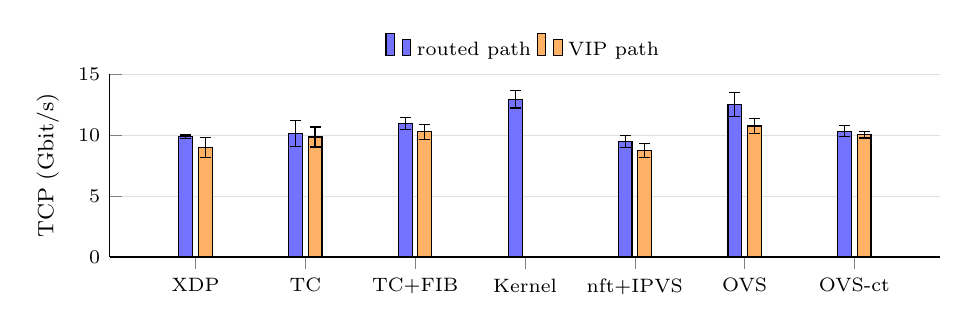
\begin{tikzpicture}
\begin{axis}[benchbar, bar width=5pt, ylabel={TCP (Gbit/s)}, ymax=15,
  nodes near coords={},
  legend style={font=\scriptsize, at={(0.5,1.02)}, anchor=south, legend columns=2, draw=none}]
\addplot[fill=blue!55, error bars/.cd, y dir=both, y explicit] coordinates {
  (XDP,9.87) +- (0,0.15) (TC,10.16) +- (0,1.07) (TC+FIB,10.96) +- (0,0.51)
  (Kernel,12.97) +- (0,0.73) (nft+IPVS,9.49) +- (0,0.51) (OVS,12.53) +- (0,0.98)
  (OVS-ct,10.33) +- (0,0.46)};
\addplot[fill=orange!60, error bars/.cd, y dir=both, y explicit] coordinates {
  (XDP,9.01) +- (0,0.82) (TC,9.86) +- (0,0.82) (TC+FIB,10.28) +- (0,0.60)
  (Kernel,0) (nft+IPVS,8.75) +- (0,0.61) (OVS,10.76) +- (0,0.59)
  (OVS-ct,10.03) +- (0,0.25)};
\legend{routed path, VIP path}
\end{axis}
\end{tikzpicture}\\[1mm]
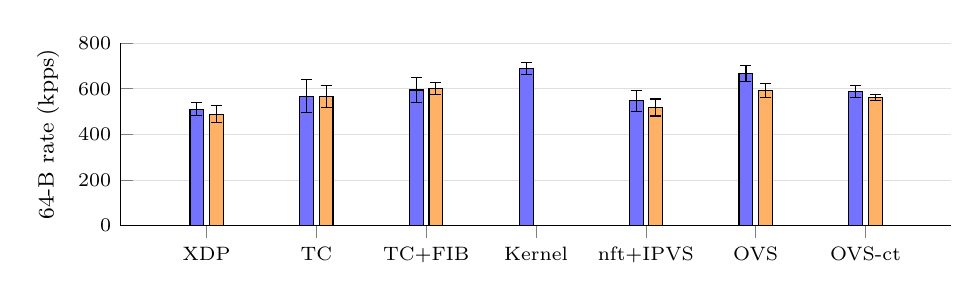
\begin{tikzpicture}
\begin{axis}[benchbar, bar width=5pt, ylabel={64-B rate (kpps)}, ymax=800,
  nodes near coords={}]
\addplot[fill=blue!55, error bars/.cd, y dir=both, y explicit] coordinates {
  (XDP,510.5) +- (0,29.5) (TC,567.7) +- (0,71.4) (TC+FIB,594.8) +- (0,56.2)
  (Kernel,688.8) +- (0,24.5) (nft+IPVS,546.9) +- (0,47.1) (OVS,667.0) +- (0,36.8)
  (OVS-ct,587.8) +- (0,27.1)};
\addplot[fill=orange!60, error bars/.cd, y dir=both, y explicit] coordinates {
  (XDP,488.3) +- (0,37.2) (TC,566.5) +- (0,47.0) (TC+FIB,600.8) +- (0,26.4)
  (Kernel,0) (nft+IPVS,518.0) +- (0,37.2) (OVS,592.7) +- (0,29.1)
  (OVS-ct,562.1) +- (0,14.2)};
\end{axis}
\end{tikzpicture}
\caption{TCP throughput (top) and received 64-byte packet rate (bottom) on
the routed path and through the VIP (kernel routing has no VIP); error bars
are 95\% confidence intervals over 10 rounds.}
\label{fig:tput}
\end{figure}

\subsection{Throughput and Packet Rate}
Table~\ref{tab:perf} lists all measurements and Fig.~\ref{fig:tput} plots
throughput and packet rate on both paths. The coefficient of variation of
TCP throughput is 2--15\% per configuration, which separates the main groups
but not every pair:
\begin{itemize}
\item \textbf{Stateless forwarding} is fastest. Kernel routing reaches
12.97~Gbit/s and 689~kpps; stateless OVS is statistically indistinguishable
from it (TCP $-3.4\%$, $p=0.42$; packet rate $-3.2\%$, $p=0.28$).
\item \textbf{Stateful processing} costs 13.6--26.9\% relative to kernel
routing in every configuration that tracks connections: OVS-ct loses 20.4\%
of TCP throughput and 14.7\% of the packet rate, nft+IPVS 26.9\% and 20.6\%,
and the eBPF data plane 15.5--23.9\% and 13.6--25.9\% (all $p<0.005$).
\item \textbf{eBPF versus the kernel's native stack.} On the routed path, XDP
and TC are statistically indistinguishable from nft+IPVS (TCP $+4.0\%$,
$p=0.13$, and $+7.1\%$, $p=0.22$), while TC+FIB is 15.5\% faster in TCP
throughput ($p<0.001$; packet rate $+8.8\%$, $p=0.16$). Through the VIP, where
both perform DNAT/SNAT, TC is 12.8\% faster than IPVS in TCP throughput
($p=0.025$) and TC+FIB 17.5\% and 16.0\% faster in TCP throughput and packet
rate ($p<0.001$).
\item \textbf{eBPF versus OVS-ct.} TC and TC+FIB are statistically
indistinguishable from OVS-ct on both paths (all $|\Delta| \le 6.1\%$,
$p \ge 0.05$), except for TC+FIB's 6.9\% higher VIP packet rate ($p=0.011$).
XDP is below OVS-ct: 13.1\% in packet rate on both paths ($p \le 0.002$) and
10.1\% in VIP TCP throughput ($p=0.022$).
\item \textbf{Hooks and forwarding.} XDP is never significantly faster than
TC; its VIP packet rate is 13.8\% lower ($p=0.009$). In-program FIB forwarding
does not significantly raise throughput over TC alone (TCP $+7.8\%$, $p=0.16$;
packet rate $+4.8\%$, $p=0.51$), but it lowers latency
(Section~\ref{sec:latency}).
\item \textbf{Cost of load balancing.} The VIP path is at most 8.7\% slower
than the routed path for every eBPF configuration, and the difference is
significant only for XDP TCP ($p=0.043$). Stateless OVS, in contrast, loses
14.1\% and 11.1\% through its \texttt{select} group ($p \le 0.003$).
\end{itemize}
These results differ from those of our first revision, in which every eBPF
configuration was 10--19\% below OVS-ct. The present version skips the rule
lookups of unpopulated patterns (Section~\ref{sec:rules}); the benchmark runs
with empty rule tables, which is the best case for this optimization.
Section~\ref{sec:kernel-cost} quantifies the cost when rules are installed.

\subsection{Latency and Connection Rate}
\label{sec:latency}
Average round-trip times are 2.1--5.5~$\mu$s, close to the 1~$\mu$s
resolution of \texttt{ping}. TC+FIB matches kernel routing (2.1~$\mu$s) and is
34\% lower than with TC alone ($p=0.002$), because the packet
leaves the gateway directly from the TC program instead of traversing the
kernel's routing path. OVS-ct has the highest average and by far the highest
maximum RTT ($486~\mu$s, with a CI as wide as its mean), and stateless OVS
reaches $152~\mu$s, versus 23--36~$\mu$s for all other configurations: the
first packet of a flow misses the OVS kernel cache and is handled by
\texttt{ovs-vswitchd} in user space. The new-connection rate through the VIP
is 1027--1319 connections/s for all load-balancing configurations, with no
significant difference between the eBPF configurations and the stateful
baselines (e.g., XDP vs.\ nft+IPVS, $p=0.88$; TC vs.\ OVS-ct, $p=0.07$); at
this level it is bounded by the user-space HTTP client and server, not by the
gateway.

\subsection{In-Kernel Cost and Scalability}
\label{sec:kernel-cost}
\textit{Rules and connections.} Fig.~\ref{fig:scale} shows the cost of an
admitted packet in the repeat loop. With empty rule tables, the pipeline costs
74~ns at XDP and 100~ns at TC; with one populated pattern
(Table~\ref{tab:paths}, pass) 93--95~ns. When rules cover all ten patterns,
every packet probes ten hash tables and the cost rises to 253--295~ns (XDP)
and 250--275~ns (TC), i.e., about 16--20~ns per populated pattern on average. The cost
then does not grow with the number of rules: from 10 to 10\,000 rules,
intermediate points vary non-monotonically within this range (e.g., 285~ns for
10 rules and 253~ns for 100 at XDP). The number of tracked connections has no
measurable effect either: 75--85~ns (XDP) and 78--82~ns (TC) from 0 to
60\,000 entries per table. This confirms the $O(1)$ claim of
Section~\ref{sec:complexity}, with a constant that depends on the number of
populated patterns, not on the number of rules.

\textit{Cache-cold state.} The repeat loop keeps one flow's state in the
cache. When 60\,000 tracked flows are visited in random order, the
single-shot cost rises from 124~ns to 682~ns at XDP and from 137~ns to 679~ns
at TC (5.5$\times$ and 4.9$\times$): the connection, reverse and telemetry
tables no longer fit the core's caches, and each lookup can miss; in
addition, the telemetry table holds only 16\,384 flows, so most packets
re-insert their telemetry entry. The hot
per-packet figures are therefore a lower bound; with many concurrent flows,
memory latency dominates.

\textit{Processing paths.} Table~\ref{tab:paths} lists the cost of each path.
Dropping costs 62--67~ns in the repeat loop, i.e., 15--16~Mpps per core of
in-kernel drop capacity, far above the 0.6--0.9~Mpps that the Python flood
generator produced. Single-shot runs include about 60--80~ns of timing
overhead (pass: 156 versus 93~ns at XDP), which cancels in differences: DNAT of
an established connection adds 56--67~ns over the pass path and SNAT
13--22~ns. The first packet of a new connection costs 2.1--2.4~$\mu$s, about
ten times an established one, because it inserts entries into the load
balancer's forward and reverse tables, the firewall's connection table and the
telemetry table. The two hooks differ by at most 16\% on any path of Table~\ref{tab:paths}.

\textit{Tail-call ablation.} Splitting the pipeline into three chained
programs, each re-parsing the packet, costs 35~ns (37\%) more on the pass
path and 69--80~ns (33--47\%) more on the DNAT and SNAT paths; a packet
dropped by the first stage costs only 3~ns (5\%) more. This quantifies the
benefit of the single-program design for this pipeline; it does not measure
Polycube or bpf-iptables themselves, which also differ in parsing and state
layout.

\textit{Control-plane cost.} One reaper sweep over $3\times60\,000$ entries
takes 0.82~s ($2.2\times10^5$ entries/s), because entries are read one system
call at a time. With full tables (Table~\ref{tab:maps}) a sweep therefore
takes about 0.9~s of the 2~s reaper period on one core; batched map
operations would reduce this.

\begin{figure}[t]
\centering
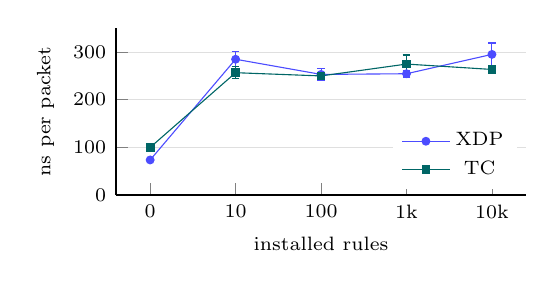
\begin{tikzpicture}
\begin{axis}[width=0.56\columnwidth, height=3.7cm, ymin=0, ymax=350,
  symbolic x coords={0,10,100,1k,10k}, xtick=data, ylabel={ns per packet},
  xlabel={installed rules}, axis lines*=left, ymajorgrids, grid style={gray!25},
  tick label style={font=\scriptsize}, label style={font=\scriptsize},
  legend style={font=\scriptsize, at={(0.98,0.03)}, anchor=south east, draw=none}]
\addplot[blue!70, mark=*, mark size=1.4pt, error bars/.cd, y dir=both, y explicit]
  coordinates {(0,73.6) +- (0,1.6) (10,284.9) +- (0,15.4) (100,253.1) +- (0,12.0)
               (1k,254.5) +- (0,6.9) (10k,295.1) +- (0,23.8)};
\addplot[teal!80!black, mark=square*, mark size=1.4pt, error bars/.cd, y dir=both, y explicit]
  coordinates {(0,99.9) +- (0,5.6) (10,256.7) +- (0,12.1) (100,249.9) +- (0,1.8)
               (1k,274.8) +- (0,19.1) (10k,263.5) +- (0,8.1)};
\legend{XDP, TC}
\end{axis}
\end{tikzpicture}%
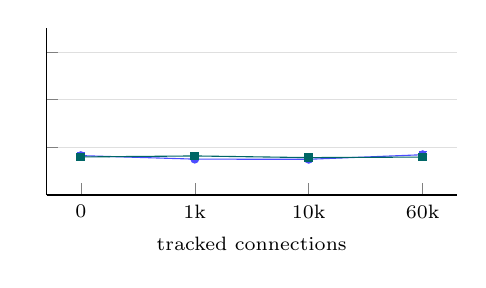
\begin{tikzpicture}
\begin{axis}[width=0.56\columnwidth, height=3.7cm, ymin=0, ymax=350,
  symbolic x coords={0,1k,10k,60k}, xtick=data, yticklabels={},
  xlabel={tracked connections}, axis lines*=left, ymajorgrids, grid style={gray!25},
  tick label style={font=\scriptsize}, label style={font=\scriptsize}]
\addplot[blue!70, mark=*, mark size=1.4pt, error bars/.cd, y dir=both, y explicit]
  coordinates {(0,82.7) +- (0,7.4) (1k,75.3) +- (0,1.1) (10k,75.0) +- (0,1.9)
               (60k,84.6) +- (0,7.1)};
\addplot[teal!80!black, mark=square*, mark size=1.4pt, error bars/.cd, y dir=both, y explicit]
  coordinates {(0,79.9) +- (0,0.9) (1k,82.0) +- (0,1.3) (10k,78.5) +- (0,0.7)
               (60k,79.7) +- (0,0.7)};
\end{axis}
\end{tikzpicture}
\caption{In-kernel cost of an admitted packet versus installed rules, spread
over all ten patterns (left; 0 rules: no populated pattern), and versus
tracked connections per table with empty rule tables (right); mean $\pm$ 95\%
CI of 15 repeat-loop samples of $2\times10^5$ runs each (performance core,
fixed governor).}
\label{fig:scale}
\end{figure}

\begin{table}[t]
\caption{In-kernel cost per processing path with one installed rule (ns,
mean $\pm$ 95\% CI; n/m: not measured)}
\label{tab:paths}
\centering\scriptsize
\setlength{\tabcolsep}{2.2pt}
\begin{tabular}{@{}lrrrrrr@{}}
\toprule
 & \multicolumn{2}{c}{Repeat loop} & \multicolumn{4}{c}{Single-shot (incl.\ timing overhead)} \\
\cmidrule(lr){2-3}\cmidrule(l){4-7}
Variant & Pass & Drop & Pass & DNAT est. & DNAT new & SNAT est. \\
\midrule
XDP & 93.3$\pm$1.8 & 61.9$\pm$0.8 & 155.7$\pm$5.1 & 211.5$\pm$6.3 & 2065$\pm$118 & 169.2$\pm$3.6 \\
TC  & 95.3$\pm$0.8 & 66.7$\pm$0.6 & 173.0$\pm$3.2 & 240.3$\pm$4.4 & 2361$\pm$157 & 195.2$\pm$2.8 \\
XDP chain & 127.9$\pm$1.2 & 65.1$\pm$1.1 & n/m & 280.5$\pm$9.0 & n/m & 249.3$\pm$7.2 \\
\bottomrule
\multicolumn{7}{@{}l}{\scriptsize XDP chain: three programs linked by \texttt{bpf\_tail\_call} (ablation (e)).}
\end{tabular}
\end{table}

\textit{Flood test.} Every flood packet was dropped in every configuration,
so the flood rates in Table~\ref{tab:perf} are bounded by the single-threaded
sender. On veth links, however, the gateway's processing runs in the
sender's softirq context on the same core, so the rate still reflects the
cost of the drop path: nft+IPVS, which drops in the forward hook after the
routing decision and the conntrack lookup, sustains 26--28\% lower rates than
the eBPF and OVS-ct data planes, which drop earlier (equivalently, these are
34--39\% faster; $p<0.001$). Among the
latter, the differences are within 3.1\% and not significant ($p \ge 0.26$).

\subsection{Discussion}
\textit{Functionality.} With connection tracking, all three stateful designs
provide the required functions: stateful filtering, VIP load balancing with
NAT, graceful draining and in-kernel drop counters. The eBPF design differs in
\emph{how}: one verified program and one set of maps implement the whole
policy, its behaviour is specified by
Eqs.~(\ref{eq:patterns})--(\ref{eq:expiry}), it exports per-flow counters of
admitted traffic, it judges load-balanced traffic by the client-visible flow,
and it isolates backend service endpoints from direct access. Stateless
OpenFlow~1.3 lacks connection tracking and drains only by re-hashing existing
connections; OVS's conntrack extensions remove this gap.

\textit{Performance.} On veth links, with sparse rule sets, the eBPF data
plane at the TC hook performs on par with OVS-ct and at least as well as the
kernel's nft+IPVS stack, and it is faster than IPVS through the VIP. Three
effects shape these numbers. First, XDP's advantage comes from running in the
NIC driver before a socket buffer is allocated; a veth packet already has
one, so native veth XDP must convert it and gains nothing from early
execution---here it is the slowest eBPF variant. Second, the per-packet cost
grows with the number of populated rule patterns (16--20~ns each), so a
policy that uses all ten patterns costs 150--220~ns more per packet than
our benchmark configuration; OVS resolves most packets with one lookup in its
megaflow cache, which already embeds the conntrack state. A per-flow verdict
cache is the corresponding optimization for the eBPF design. Third, with
many concurrent flows memory latency, not instruction count, dominates the
cost (Section~\ref{sec:kernel-cost}).

\subsection{Threats to Validity}
\label{sec:threats}
All links are veth pairs inside one machine, which does not exercise XDP's
driver-level fast path, and the traffic generators share the CPU with the
gateway; pinning and interleaving reduce but do not remove this interference.
Ten rounds bound the uncertainty of each mean (Table~\ref{tab:perf}); smaller
differences, such as among the three eBPF configurations, remain within it,
and we do not correct for multiple comparisons. The macro-benchmarks use
empty rule tables, which favours the eBPF design (Section~\ref{sec:kernel-cost}
gives the cost with rules). Disabling checksum offload lowers absolute TCP
throughput equally for all configurations. The HTTP connection rate is
bounded by Python servers, and the flood rate by a Python sender. The
microbenchmark measures the program alone, without driver and stack costs,
and its repeat loop keeps state hot in the cache. The T3 distribution test
has low statistical power, which the in-kernel test (f) compensates for.

%=====================================================================
\section{Conclusion}
%=====================================================================
We designed, implemented and evaluated an eBPF/XDP gateway data plane that
moves the SDN switch into the Linux kernel. One verified pipeline provides a
stateful firewall over the client-visible flow, an L4 load balancer with
DNAT/SNAT, graceful draining that spreads a drained backend's share evenly,
recovery of evicted NAT state and $O(1)$ checksum maintenance, and per-flow
telemetry at either the XDP or the TC hook; a libbpf-based control plane
reprograms it at runtime and expires connection state like OpenFlow
timeouts. The implementation passes 115 of 116 automated unit and kernel
tests (one skipped because of a kernel test-harness limitation) and every
end-to-end scenario at both hooks. In 10 interleaved, pinned rounds on
emulated veth links and with sparse rule sets, it reaches 9.9--11.0~Gbit/s
of TCP throughput and 511--595~kpps for 64-byte packets on the routed path
(13.6--25.9\% below plain kernel routing), and 9.0--10.3~Gbit/s and
488--601~kpps through the load balancer. At the TC hook this is
statistically indistinguishable from OVS with connection tracking, and with
in-program FIB forwarding 16--18\% faster than nftables with IPVS through
the VIP. Measured in the kernel, an admitted packet costs 74--100~ns with
empty rule tables and 250--295~ns when all ten rule patterns are populated,
independent of the number of rules (10--10\,000) and tracked connections
(0--60\,000); with 60\,000 flows in random order, cache misses raise it to
about 0.68~$\mu$s. A dropped packet costs 62--67~ns, and splitting the
pipeline into tail-called programs adds 33--47\% on the pass and NAT paths.
Future work will evaluate the system on physical NICs with native XDP support
and hardware traffic generators, add a per-flow verdict cache to remove the
per-pattern cost, replace the active-list modulo selection with Maglev-style
consistent hashing \cite{eisenbud2016maglev} to reduce remapping when pools
change, use batched map operations in the reaper, and add prefix (LPM) rules.

%=====================================================================
\input{appendix_figs}

%=====================================================================
\begin{thebibliography}{00}
\bibitem{kreutz2015sdn} D. Kreutz, F. M. V. Ramos, P. E. Ver\'issimo,
C. E. Rothenberg, S. Azodolmolky, and S. Uhlig, ``Software-defined networking:
A comprehensive survey,'' \textit{Proc. IEEE}, vol.~103, no.~1, pp.~14--76,
Jan. 2015, doi: 10.1109/JPROC.2014.2371999.

\bibitem{feamster2014road} N. Feamster, J. Rexford, and E. Zegura, ``The road
to SDN: An intellectual history of programmable networks,'' \textit{ACM
SIGCOMM Comput. Commun. Rev.}, vol.~44, no.~2, pp.~87--98, Apr. 2014,
doi: 10.1145/2602204.2602219.

\bibitem{mckeown2008openflow} N. McKeown, T. Anderson, H. Balakrishnan,
G. Parulkar, L. Peterson, J. Rexford, S. Shenker, and J. Turner, ``OpenFlow:
Enabling innovation in campus networks,'' \textit{ACM SIGCOMM Comput. Commun.
Rev.}, vol.~38, no.~2, pp.~69--74, Apr. 2008, doi: 10.1145/1355734.1355746.

\bibitem{pfaff2015ovs} B. Pfaff, J. Pettit, T. Koponen, E. Jackson, A. Zhou,
J. Rajahalme, J. Gross, A. Wang, J. Stringer, P. Shelar, K. Amidon, and
M. Casado, ``The design and implementation of Open vSwitch,'' in \textit{Proc.
12th USENIX Symp. Netw. Syst. Design Implement. (NSDI)}, Oakland, CA, USA,
2015, pp.~117--130.

\bibitem{hoiland2018xdp} T. H{\o}iland-J{\o}rgensen, J. D. Brouer,
D. Borkmann, J. Fastabend, T. Herbert, D. Ahern, and D. Miller, ``The eXpress
data path: Fast programmable packet processing in the operating system
kernel,'' in \textit{Proc. 14th Int. Conf. Emerg. Netw. Exp. Technol.
(CoNEXT)}, Heraklion, Greece, 2018, pp.~54--66, doi: 10.1145/3281411.3281443.

\bibitem{vieira2020ebpf} M. A. M. Vieira, M. S. Castanho, R. D. G. Pac\'ifico,
E. R. S. Santos, E. P. M. C\^amara J\'unior, and L. F. M. Vieira, ``Fast packet
processing with eBPF and XDP: Concepts, code, challenges, and applications,''
\textit{ACM Comput. Surv.}, vol.~53, no.~1, pp.~1--36, Feb. 2020,
doi: 10.1145/3371038.

\bibitem{cilium} Cilium Authors, ``Cilium: eBPF-based networking,
observability, and security,'' 2025. [Online]. Available:
https://cilium.io (accessed Nov. 17, 2026).

\bibitem{katran} Meta Platforms, ``Katran: A high performance layer 4 load
balancer,'' 2025. [Online]. Available:
https://github.com/facebookincubator/katran (accessed Nov. 17, 2026).

\bibitem{miano2021polycube} S. Miano, F. Risso, M. V. Bernal, M. Bertrone, and
Y. Lu, ``A framework for eBPF-based network functions in an era of
microservices,'' \textit{IEEE Trans. Netw. Service Manag.}, vol.~18, no.~1,
pp.~133--151, Mar. 2021, doi: 10.1109/TNSM.2021.3055676.

\bibitem{bosshart2014p4} P. Bosshart, D. Daly, G. Gibb, M. Izzard,
N. McKeown, J. Rexford, C. Schlesinger, D. Talayco, A. Vahdat, G. Varghese,
and D. Walker, ``P4: Programming protocol-independent packet processors,''
\textit{ACM SIGCOMM Comput. Commun. Rev.}, vol.~44, no.~3, pp.~87--95,
Jul. 2014, doi: 10.1145/2656877.2656890.

\bibitem{tu2021ovs} W. Tu, Y.-H. Wei, G. Antichi, and B. Pfaff, ``Revisiting
the Open vSwitch dataplane ten years later,'' in \textit{Proc. ACM SIGCOMM
Conf.}, 2021, pp.~245--257, doi: 10.1145/3452296.3472914.

\bibitem{chaignon2018oko} P. Chaignon, K. Lazri, J. Fran\c{c}ois, T. Delmas,
and O. Festor, ``Oko: Extending Open vSwitch with stateful filters,'' in
\textit{Proc. Symp. SDN Res. (SOSR)}, Los Angeles, CA, USA, 2018, pp.~1--13,
doi: 10.1145/3185467.3185496.

\bibitem{miano2018creating} S. Miano, M. Bertrone, F. Risso, M. Tumolo, and
M. V. Bernal, ``Creating complex network services with eBPF: Experience and
lessons learned,'' in \textit{Proc. IEEE 19th Int. Conf. High Perform.
Switching Routing (HPSR)}, Bucharest, Romania, 2018, pp.~1--8,
doi: 10.1109/HPSR.2018.8850758.

\bibitem{miano2019bpfiptables} S. Miano, M. Bertrone, F. Risso, M. V. Bernal,
Y. Lu, and J. Pi, ``Securing Linux with a faster and scalable iptables,''
\textit{ACM SIGCOMM Comput. Commun. Rev.}, vol.~49, no.~3, pp.~2--17,
Jul. 2019, doi: 10.1145/3371927.3371929.

\bibitem{scholz2018filtering} D. Scholz, D. Raumer, P. Emmerich, A. Kurtz,
K. Lesiak, and G. Carle, ``Performance implications of packet filtering with
Linux eBPF,'' in \textit{Proc. 30th Int. Teletraffic Congr. (ITC)}, Vienna,
Austria, 2018, pp.~209--217, doi: 10.1109/ITC30.2018.00039.

\bibitem{nftables} Netfilter Project, ``nftables,'' 2025. [Online].
Available: https://netfilter.org/projects/nftables/ (accessed Nov. 17, 2026).

\bibitem{zhang2000lvs} W. Zhang, ``Linux Virtual Server for scalable network
services,'' in \textit{Proc. Ottawa Linux Symp.}, Ottawa, ON, Canada,
Jul. 2000.

\bibitem{eisenbud2016maglev} D. E. Eisenbud, C. Yi, C. Contavalli, C. Smith,
R. Kononov, E. Mann-Hielscher, A. Cilingiroglu, B. Cheyney, W. Shang, and
J. D. Hosein, ``Maglev: A fast and reliable software network load balancer,''
in \textit{Proc. 13th USENIX Symp. Netw. Syst. Design Implement. (NSDI)},
Santa Clara, CA, USA, 2016, pp.~523--535.

\bibitem{srinivasan1999tss} V. Srinivasan, S. Suri, and G. Varghese, ``Packet
classification using tuple space search,'' in \textit{Proc. ACM SIGCOMM
Conf.}, Cambridge, MA, USA, 1999, pp.~135--146, doi: 10.1145/316188.316216.

\bibitem{lantz2010mininet} B. Lantz, B. Heller, and N. McKeown, ``A network in
a laptop: Rapid prototyping for software-defined networks,'' in \textit{Proc.
9th ACM SIGCOMM Workshop Hot Topics Netw. (HotNets)}, Monterey, CA, USA, 2010,
Art. no.~19, doi: 10.1145/1868447.1868466.

\bibitem{rfc1624} A. Rijsinghani, ``Computation of the Internet checksum via
incremental update,'' RFC 1624, IETF, May 1994, doi: 10.17487/RFC1624.

\bibitem{rfc1071} R. Braden, D. Borman, and C. Partridge, ``Computing the
Internet checksum,'' RFC 1071, IETF, Sep. 1988, doi: 10.17487/RFC1071.

\bibitem{rfc768} J. Postel, ``User datagram protocol,'' RFC 768, IETF,
Aug. 1980, doi: 10.17487/RFC0768.

\bibitem{kuo2022kfuse} H.-C. Kuo, K.-H. Chen, Y. Lu, D. Williams, S. Mohan,
and T. Xu, ``Verified programs can party: Optimizing kernel extensions via
post-verification merging,'' in \textit{Proc. 17th Eur. Conf. Comput. Syst.
(EuroSys)}, Rennes, France, 2022, pp.~283--299, doi: 10.1145/3492321.3519562.

\bibitem{miano2022morpheus} S. Miano, A. Sanaee, F. Risso, G. R\'etv\'ari,
and G. Antichi, ``Domain specific run time optimization for software data
planes,'' in \textit{Proc. 27th ACM Int. Conf. Archit. Support Program.
Lang. Oper. Syst. (ASPLOS)}, Lausanne, Switzerland, 2022, pp.~1148--1164,
doi: 10.1145/3503222.3507769.

\bibitem{nfflowtable} Linux Kernel Documentation, ``Netfilter's flowtable
infrastructure,'' 2026. [Online]. Available:
https://docs.kernel.org/networking/nf\_flowtable.html (accessed Nov. 18, 2026).
\end{thebibliography}

\end{document}
